\setchapterpreamble[u]{\margintoc}
\chapter{Intégration}
\labch{integration}

\todoinline{
Remarques générales :
}

\todoinline{Il faudrait je pense mettre les illustrations dans un sous-dossier integration/ pour qu'on s'y retrouve à terme}

\todoarmand{Les trois dernières animations du chapitre "Intégration sur un intervalle quelconque" sur votre site ne sont pas accessibles, est-ce normal ?}

\todoinline{Une erreur dans un nom de dossier. J'ai corrigé. Si tu veux les sources python, je peux te les envoyer. C'est un peu à la main et je crois qu'il y a un outil plus performant maintenant...}


\todoarmand{
Inclure le flow chart \url{https://acamanes.github.io/psi/psi_doc/fc03.pdf} ? \\
J'ai vu sur votre site que vous aviez fait plein de diagrammes pour les ECT. On pourrait inclure ceux sur l'intégration ?
}

\todoinline{Je les ai ajoutés. Je te laisse juger si ça vaut le coup de les mettre, je ne suis pas neutre sur ce sujet !}

\todoarmand{J'ai modifié les différents environnements, les seules modifications par rapport aux anciens sont: "preuve" devient "demo", "elem\_demo" devient "elemdemo" et "elem\_sol" devient "elemsolution". De plus, on peut maintenant ajouter un titre optionnel entre crochets à tous les environnements: théorème, proposition, ..., exercice, remarque, démonstration, ...}

\todoarmand{J'ai aussi introduit des environnements "questions" et "reponses" à la place des simples "enumerate".}

\todoarmand{J'ai l'impression que vous compilez le fichier main\_integration, je compile plutôt le fichier main. Ça ne change quasiment rien mais je préfère le préciser.}

\todoinline{Très bien le schéma, je le vérifierai après avoir tout relu}

\begin{figure}[H]
    \centering
    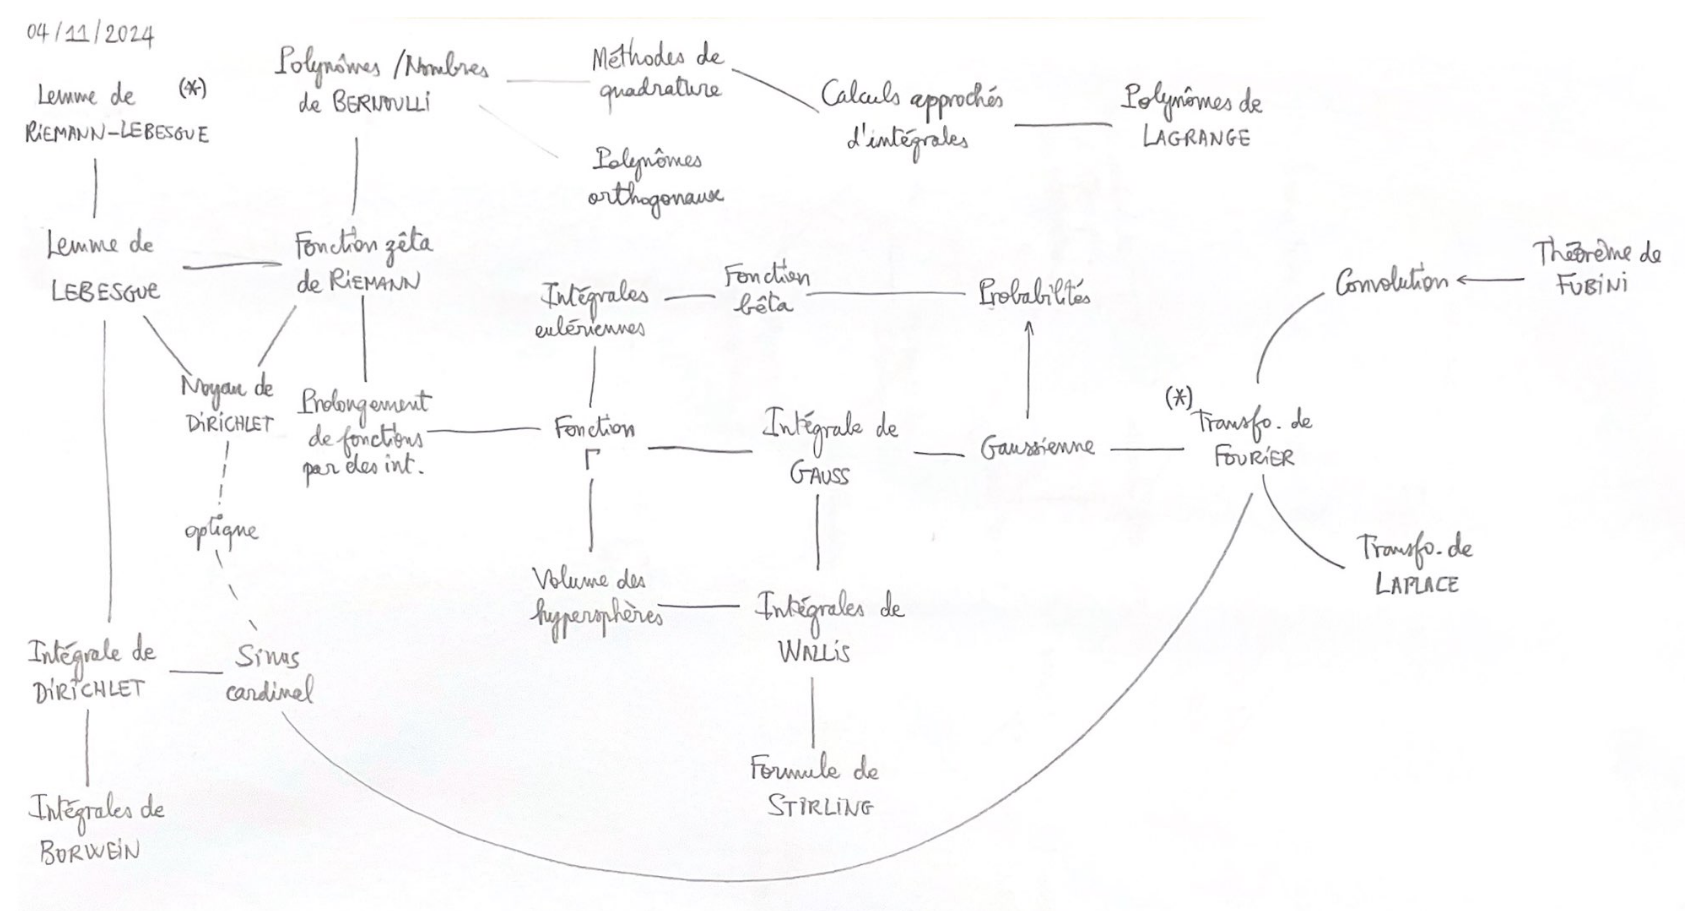
\includegraphics[width=1\linewidth]{chapitres/integration/documents/diagramme_integration.png}
    \caption{Ébauche d'un diagramme des chapitres}
\end{figure}

\todoinline{Chapitres validés : \\
01 : Changement de titre\\
02 : J'ai ajouté un encadré exercice à valider - Le titre de la figure, je le trouve bien - Les liens avec Bernoulli, ça me va mais garder l'encadrer pour rester self-contained.\\
03 : Ecadrés exercices ajoutés - Relire Simpson - Dessins à compléter\\
04 :  Ecadrés exercices ajoutés - Peut être un dessin de plus\\
05 : Ajout de propositions, correction d'une coquille\\
07 : correction de coquilles, ajout des prop/questions/réponses , Ajouter un graphique ?.\\
08 : Mise en forme - Proposition de déplacement}